% Pursuing Stacks (cotes 134-2 to 134-8): archive cote 134-4, site page 4 (PDF page 5), typescript page 92.
% typescript. Draft compared: ps3.tex:161-221.
% AI-transcribed by Claude Opus 5.5 (claude-opus-5-5, adaptive thinking, effort high), Message Batches API, batch ps1 (msgbatch_01Rv5hCaNTtUt4JHx1yqoHPL), 2026-11-12; image review recorded in records/CHECK_DECISIONS_134_3_4.tsv.
\scanpage{134-4/4}
\xout{(92)}
\mspage{(92)}
dency though to commute to sums,  as usual.

I would'nt overemphasize the capacity of (Spaces\over{'}{)} to serve the purpose
of a ``basic modelizer'' as \inserted{does} (Cat),  despite the attractive feature of more
direct (or at any rate,  more convential) ties with so-called ``topological
intuition''.  O\over[typed]{N}{n}e drawback of (Spaces) is the relative sophistication of
the structure species ``topological spaces'' it corresponds to,  which is
by no means an ``algebraic structure species'',  and fits into algebraic
formalism\hand{s} only at the price of detours.  M$\overset{\hand{\smile}}{\mathrm{o}}$re seriously still,  or rather
as a reflection of this latter feature,  only for some rather special
elementary modelizers $A^{\hand{\wedge}}$,  namely rather special test categories $A$,  do
we get a geometric realization functor $r_{\hand{!}} : A^{\hand{\wedge}} \hand{\longrightarrow} (\mathrm{Spaces})$ which \over[typed]{i}{c}\over[typed]{a}{a}n be
viewed as part of a pair of mutually adjoint modelizing functors,
mimicking the \over[typed]{p}{c}anonical pair $(i_A, j_A)$;  still \over{t}{l}\over{e}{e}ss \over[typed]{d}{d}oes there seem\deleted{s} to be
anything like a really canonical choice (although some choices are pretty
natural indeed,  dealing with the standart test categories such as \hand{$\Delta$} and
it\hand{'}s variants).  At any rate,  it is still to be seen whether there exists
such a pair  $(r_{\hand{!}}, r^{*})$  for \hand{some} rather general class\deleted{\unsure{e}} of test categories  -
this is one among the very many things that I keep pushing off,  as more
urgent matters are calling for attention ...

To sum up the outcome of these unformal reflections \deleted{upon} \inserted{about} various
types of modelizing functors between modelizers,  the two main types which
seem to overtower the whole picture,  and are likely to be the essential
ones for a general understanding of homotopy models,  are the two types
(1) and (2)  above.  T\over[typed]{H}{h}e first one $i^{*}$ is defined in terms of an arbitrary
test functor (still to be 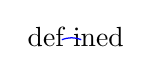
\begin{tikzpicture}[baseline=(w.base)]\node[inner sep=0pt] (w) {def ined};\draw[color=blue,line width=.45pt] ([xshift=-.5em,yshift=.65ex]w.south) to[bend left=20] ([xshift=.2em,yshift=.65ex]w.south);\end{tikzpicture} !)  of a test category into an arbitra-%
ry\xout{x} modelizer $M$.  The second $i_A$ ,  with opposite exactness properties to
the previous one,  is canonically attached to any test category,  and
\xout{ties} maps the corresponding elementary modelizer  $A^{\hand{\wedge}}$ into the basic mode-%
lizer (Cat),  without any reference to more general types of modelizers $M$.
The right adjoint of the latter,  which is still model preserving,  is
in fact of the type (1) again,  for the canonical test functor $A \hand{\longrightarrow} (\mathrm{Cat})$
induced by $i_A$ ,  namely $a \hand{\mapsto} A_{\hand{/}a}$ .  \begin{tikzpicture}[baseline=-.2ex]\draw[color=blue] (0,0)--(.45,0)--(.45,.4)--(.82,.4);\draw[color=blue] (.49,.02)--(.49,.42);\end{tikzpicture} T\over[typed]{H}{h}\over{e}{is} whole reflection was of course on
such an unformal level,  that there was no sense at that stage to bother
with distinctions between weaker or stricter  variants of the test-notions
Maybe it's about time now to start getting a little more specific.

\margin{4}
